
\begin{figure}[ht]
\centering
\begin{tabular}{| l | l | c |}
  \hline
  ID & Description & Link \\
  \hline
  1 & Single Agent Results, coloured by opposite surface& \href{https://barrett370.github.io/Y4-Diss/single-agent-result-1404-col}{url} \\
  2 & Multi agent results & \href{https://barrett370.github.io/Y4-Diss/multi-agent-result-1304}{url} \\
  3 & Multi agent results, coloured by opposite surface & \href{https://barrett370.github.io/Y4-Diss/multi-agent-result-1904-col}{url} \\
  4 & Multi agent results, coloured by opposite surface, fitness threshold = 40 & \href{https://barrett370.github.io/Y4-Diss/multi-agent-result-1304-lim40-col}{url} \\
  5 & Multi agent results, with fitness-planning time overlayed, fitness threshold=100 & \href{https://barrett370.github.io/Y4-Diss/multi-agent-result-shared-lim100}{url} \\


  \hline
\end{tabular}
\caption{\label{tab:plotlinks} External links to dynamic plots}
\end{figure}\feedback{Is this a clear way of formatting? I would reference the ID when talking about a plot. I would still include an image as a figure}

Due to the high dimensionality of my search space, I cannot visualise the objective function of my GA.

\begin{figure}[ht]
  \centering
  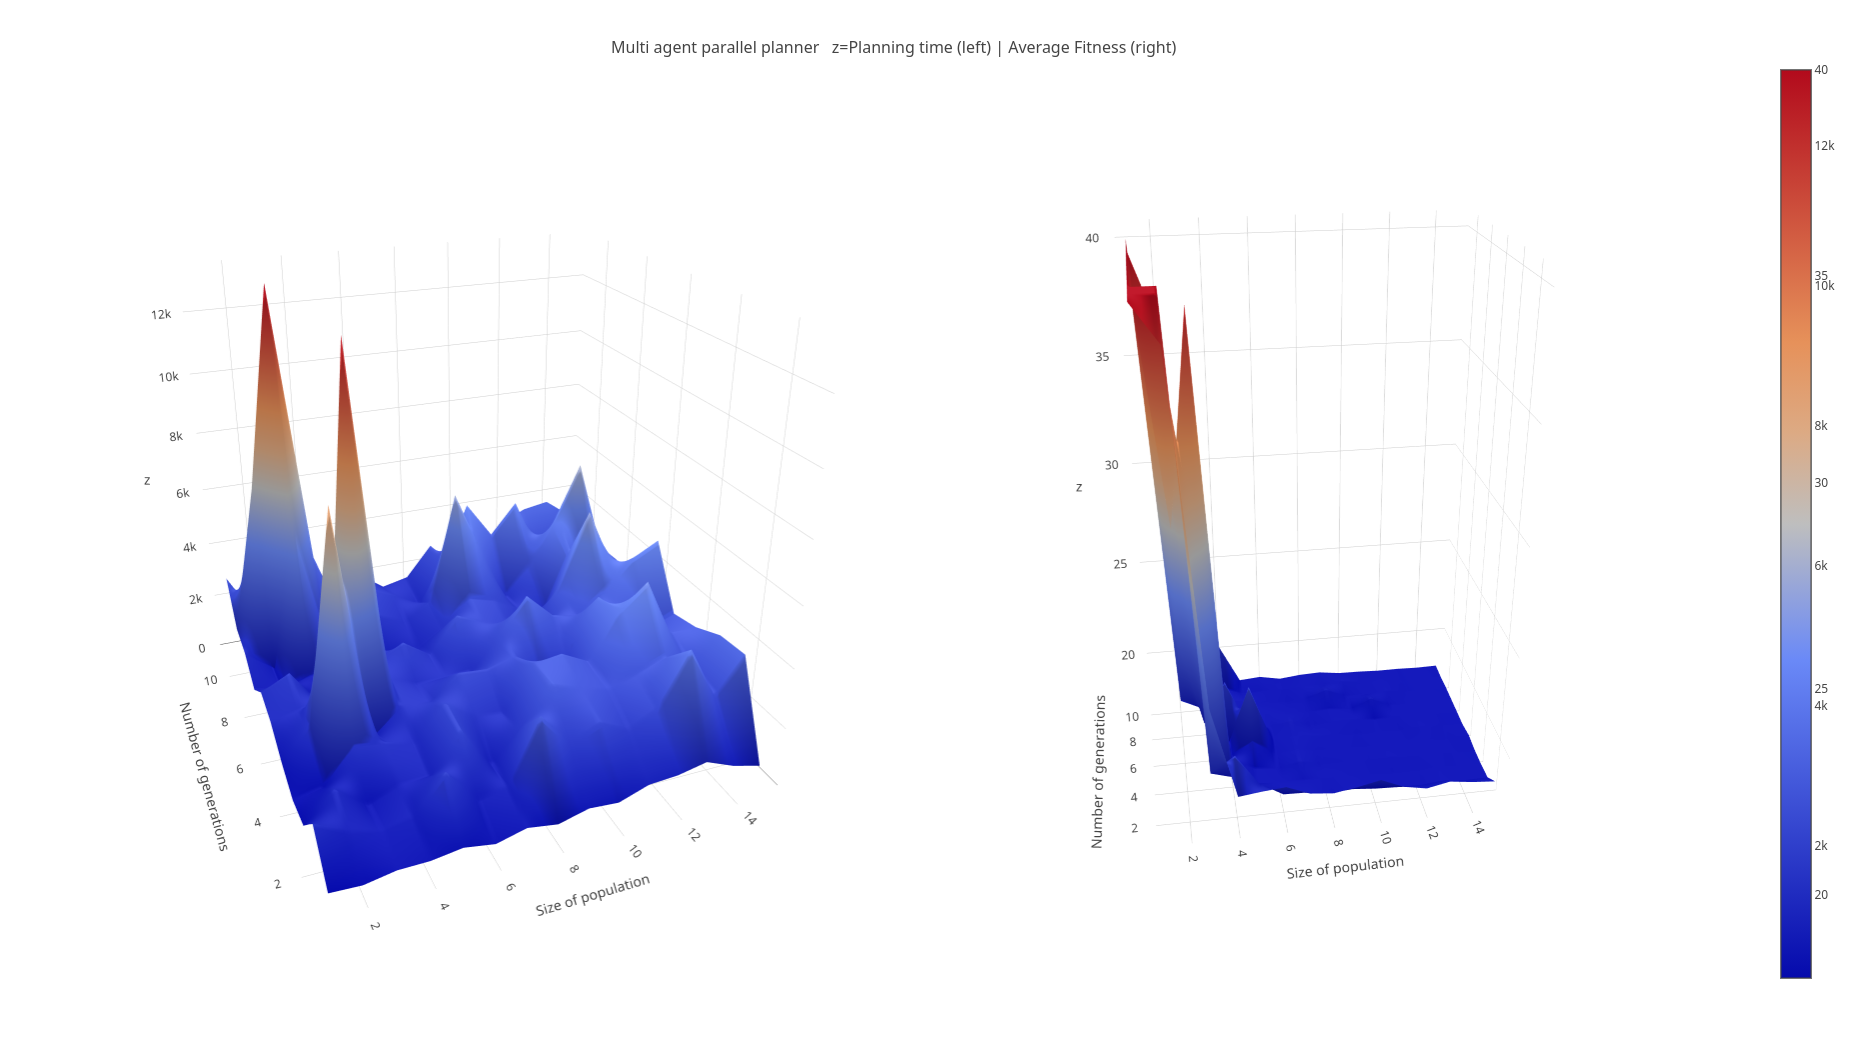
\includegraphics[scale=0.19]{figures/ma-1304-lim40.png}
  \caption{\label{fig:ma-lim40} Multi agent planning number of generations against size of population against planning time (left), fitness limited at 40 (right)}
\end{figure}
\todo{Check units for planning time + add link to hosted dynamic version}

\begin{figure}[ht]
  \centering
  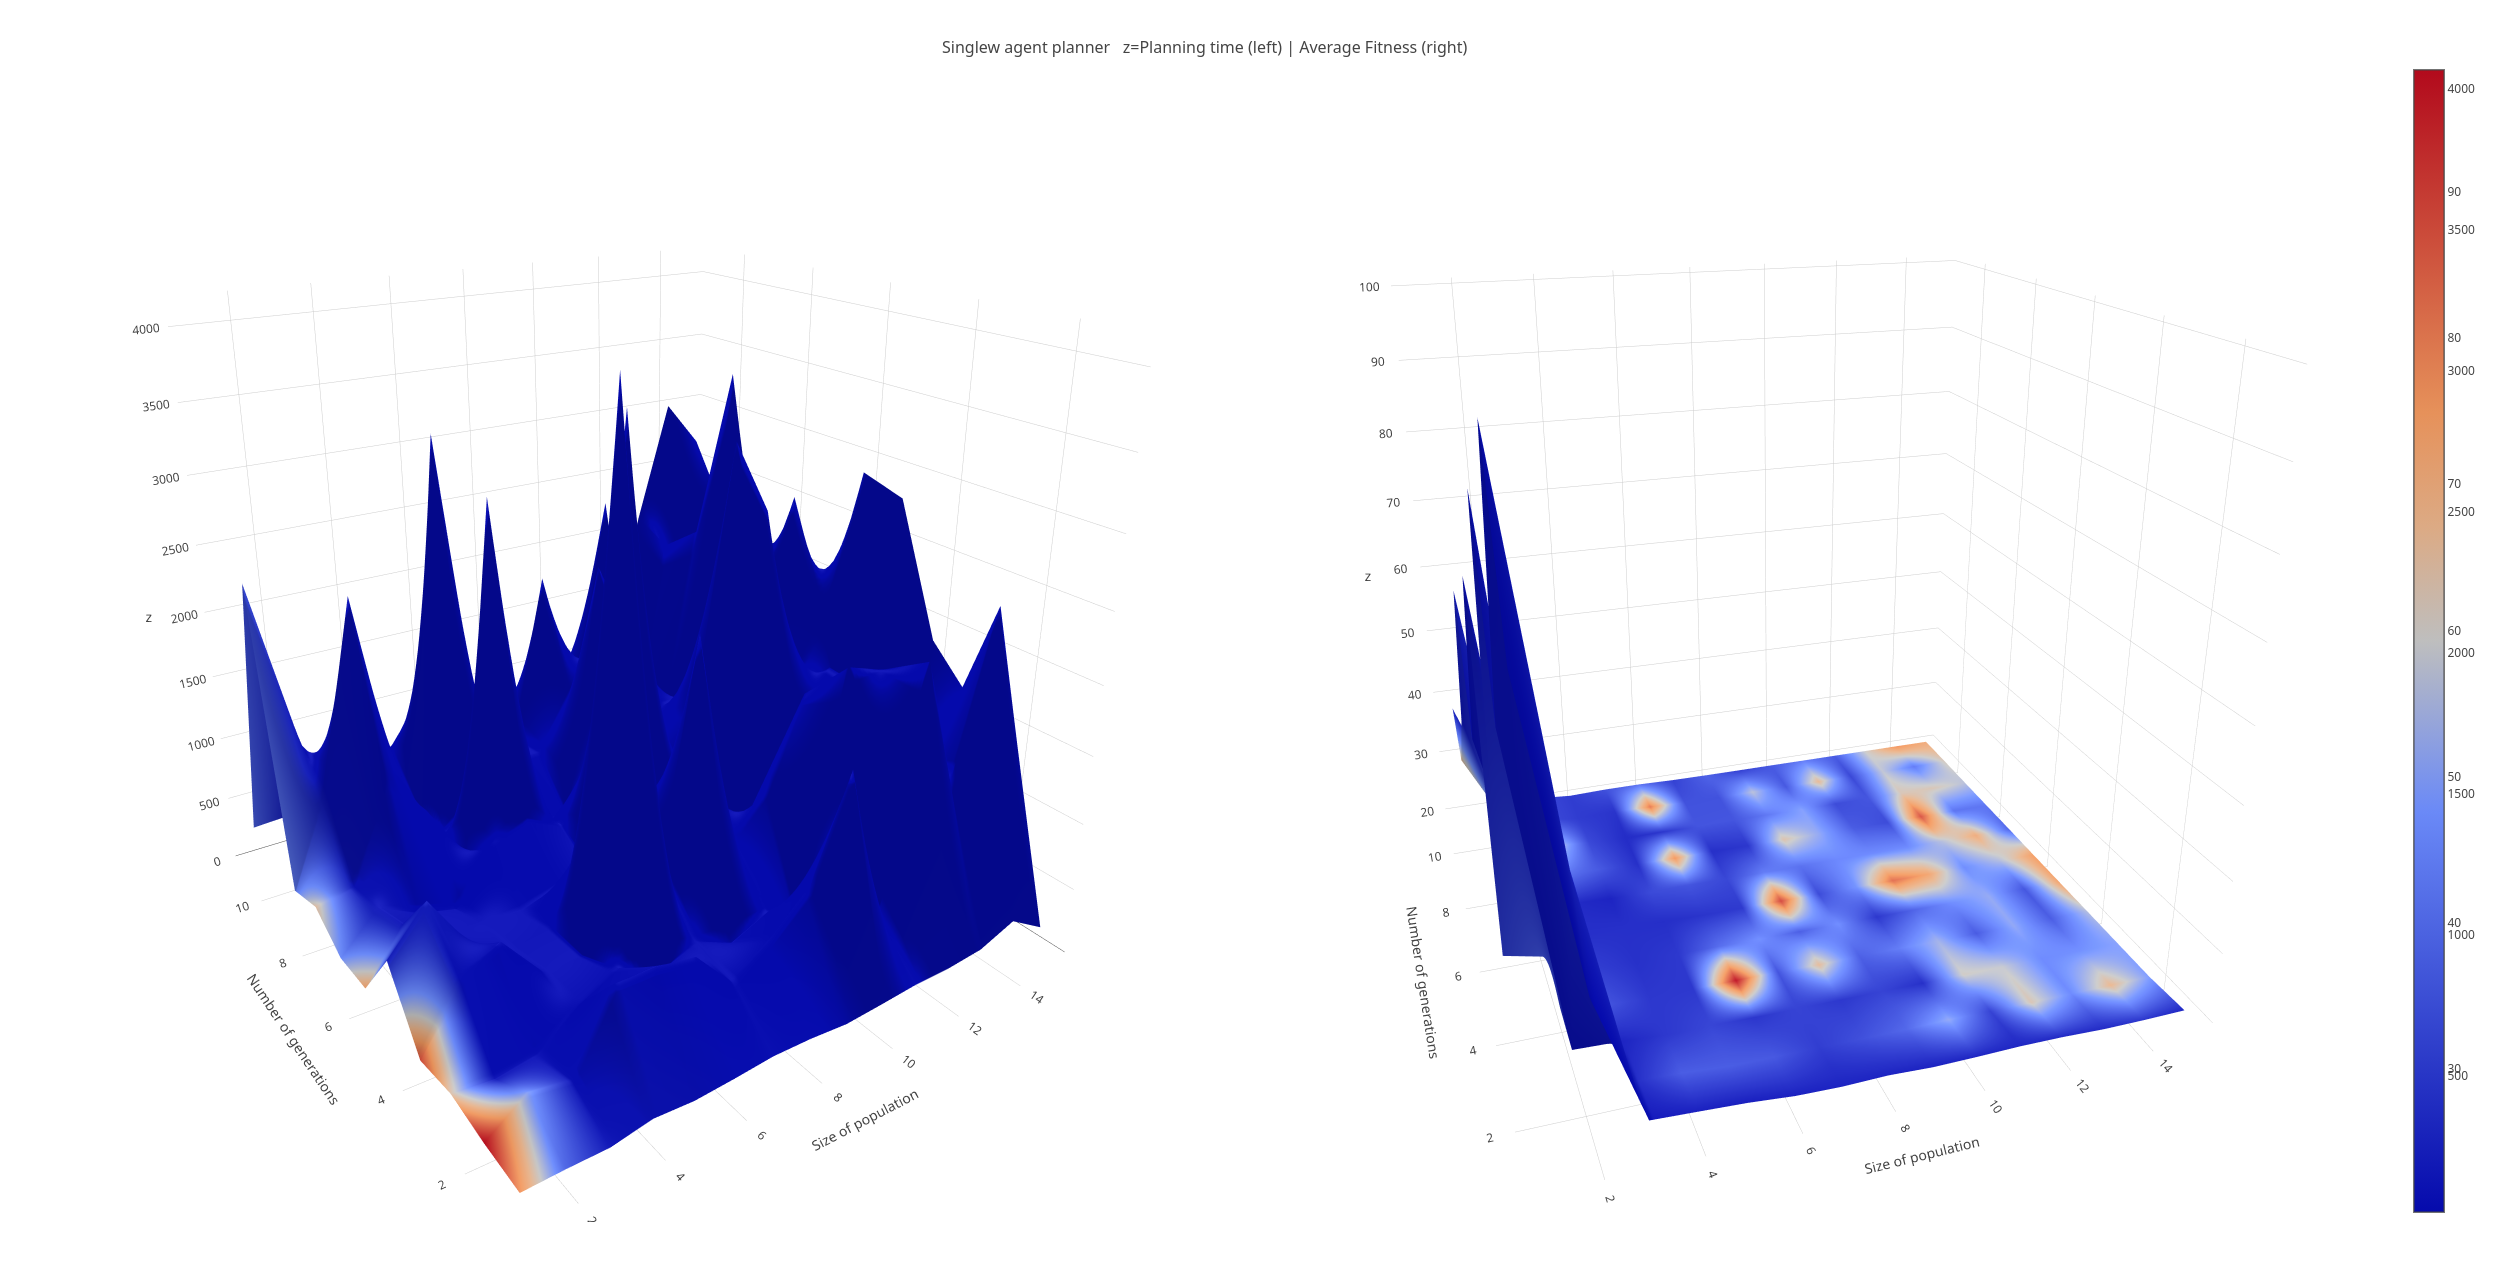
\includegraphics[scale=0.14]{figures/sa-1404-col.png}
  \caption{\label{fig:sa-col} Single agent planning: number of generations against size of population against planning time (left), fitness (right)}
\end{figure}
\todo{Check units for planning time + add link to hosted dynamic version}
